\documentclass[11pt,a4paper]{article}

% ---------------------------------------------------------------------------
% Permanence and composition control for self-limited consumers coupled to a
% dynamic resource network.
%
% Author metadata: set the three macros below before submission.
% They are deliberately left blank in this version.
% ---------------------------------------------------------------------------
\newcommand{\PaperAuthor}{}
\newcommand{\PaperAffiliation}{}
\newcommand{\PaperDate}{14 September 2026}

\usepackage[T1]{fontenc}
\usepackage[utf8]{inputenc}
\usepackage{lmodern}
\usepackage{microtype}
\usepackage[a4paper,margin=1.05in]{geometry}
\usepackage{amsmath,amssymb,amsthm,mathtools}
\usepackage{booktabs}
\usepackage{array}
\usepackage{enumitem}
\usepackage{capt-of}
\usepackage{xcolor}
\usepackage{graphicx}
\usepackage[obeyspaces,spaces]{url}
\usepackage[numbers,sort&compress]{natbib}
\usepackage[colorlinks=true,linkcolor=blue!55!black,citecolor=blue!55!black,urlcolor=blue!55!black]{hyperref}
\hypersetup{pdftitle={Permanence and composition control for self-limited consumers coupled to a dynamic resource network},
  pdfkeywords={permanence, uniform persistence, competition for a single resource, intraspecific regulation, chemical reaction networks, mass action, autocatalytic networks, Lean}}

\DeclareUrlCommand\lean{\urlstyle{tt}}
\setlist{itemsep=2pt,topsep=3pt}
\setlength{\emergencystretch}{1.5em}
\graphicspath{{figures/}}

\theoremstyle{plain}
\newtheorem{theorem}{Theorem}[section]
\newtheorem{proposition}[theorem]{Proposition}
\newtheorem{lemma}[theorem]{Lemma}
\newtheorem{corollary}[theorem]{Corollary}
\theoremstyle{definition}
\newtheorem{definition}[theorem]{Definition}
\theoremstyle{remark}
\newtheorem{remark}[theorem]{Remark}

\newcommand{\R}{\mathbb R}
\newcommand{\D}{\mathcal D}
\newcommand{\cE}{\mathcal E}
\newcommand{\avg}[1]{\overline{#1}_T}
\newcommand{\norm}[1]{\left\lVert#1\right\rVert}
\newcommand{\abs}[1]{\left|#1\right|}
\newcommand{\eps}{\varepsilon}
\newcommand{\dd}{\mathrm d}
\DeclareMathOperator{\diag}{diag}

\title{Permanence and composition control for self-limited consumers coupled to a dynamic resource network}
\author{\PaperAuthor\\[2pt]{\small\itshape\PaperAffiliation}}
\date{\PaperDate}

\begin{document}
\maketitle

\begin{abstract}
We study finitely many consumers that copy themselves from a shared resource, are each separately self-limited, and are coupled to a four-variable mass-action network that produces the resource. We prove positive global existence and uniform permanence from every strictly positive initial state, first with a maintained copying precursor and then with an explicitly consumed, replenished reservoir. The conclusions hold for every number $n\ge2$ of consumers, on a reference parameter interval, and on a full neighborhood in which every directed reaction rate varies independently. No equilibrium, convergence, invasion-rate, or fast-reservoir assumption is imposed on the resource network. The proof combines a bounded resident potential, a quadratic reservoir correction, and a scalar quotient comparison that converts persistence of the total consumer abundance into persistence of every individual consumer; the comparison yields an individual floor that is linear in the aggregate floor. For the reference normalization, composition restoration then gives a floor of order $1/n$ with a constant independent of $n$. We also establish a source-level extension in which arbitrary positive self-limitation coefficients prescribe arbitrary target proportions, time-averaged supply and finite-inventory bounds, a small-supply stationary branch, an exact rational local operating certificate, and a negative control showing that removing self-limitation restores competitive exclusion. The five source endpoints, the sharpened recovery bounds, the composition consequences and the negative control are checked in Lean~4 against the literal mass-action field; the remaining analytic consequences and rational certificates have conventional proofs given here. The model is an effective, externally supplied reaction system, not a thermodynamic or finite-population realization.
\end{abstract}

\section{Introduction}\label{sec:intro}

\subsection{Setting and question}
When several populations grow on one limiting resource, the competitive exclusion principle predicts that at most one survives at equilibrium \cite{Hardin1960,HsuHubbellWaltman1977,SmithWaltman1995}. Coexistence requires an additional mechanism: nonequilibrium dynamics \cite{ArmstrongMcGehee1980}, or a stabilizing difference between intraspecific and interspecific regulation \cite{Chesson2000}. In chemostat theory the second mechanism has been made precise: when each species is limited by its own density in addition to the shared resource, $n$ species can coexist on a single resource \cite{LobryMazencRapaport2005,LobryHarmand2006}, and Abdellatif, Fekih-Salem and Sari give coexistence conditions, operating diagrams and a global stability analysis for a density-dependent chemostat model \cite{AbdellatifFekihSalemSari2016}.

The present paper asks the same question in a different resource environment. The resource is not a chemostat nutrient with a fixed inflow, but the output of an interacting four-variable reaction network that is itself loaded by the consumers, has no assumed equilibrium, and whose response to consumption is nonlinear. In a second stage, the copying reaction additionally consumes a precursor $R$ drawn from a reservoir that is depleted by copying and replenished by exchange with the exterior. The consumers are $n$ copying species $X_1,\dots,X_n$, each with its own copying channel $X_i+z\to2X_i$ (or $X_i+z+R\to2X_i$), its own linear loss, and its own quadratic self-limitation $2X_i\to X_i$. There is no immigration: every consumer extinction face is invariant, and a consumer that is initially rare must recover from arbitrarily small abundance.

This network is an effective description of a copying subsystem coupled to a resource-producing core of the kind studied in the theory of reflexively autocatalytic food-generated (RAF) networks \cite{Kauffman1986,HordijkSteel2004,HordijkSteel2018,SteelHordijkXavier2019}. RAF theory is structural: it identifies which sets of reactions are collectively self-sustaining given a food source. Whether a structurally autocatalytic set is also dynamically permanent, that is, whether every one of its species stays bounded away from extinction along every positive trajectory, is a separate question in the dynamics of mass-action systems \cite{AngeliDeLeenheerSontag2007,CraciunNazarovPantea2013,Feinberg2019}. This paper answers that question for one explicit family.

\subsection{Main results}
Write $S=\sum_iX_i$ for the total consumer abundance. The main results are as follows; the precise statements are Theorems~\ref{thm:roots}--\ref{thm:supply} and Propositions~\ref{prop:negative}--\ref{prop:local}.
\begin{enumerate}[label=(\roman*)]
\item \emph{Permanence with a maintained precursor} (Theorem~\ref{thm:roots}, A1--A2). For every $n\ge2$ the system with $n$ consumers has a unique global positive solution from every strictly positive initial state, and there is a floor $\eta(n)>0$ such that every physical coordinate is eventually at least $\eta(n)$, uniformly over the reference parameter interval and all positive initial states. The same holds on a full cube of independently varying directed reaction rates, of positive radius, around every reference point.
\item \emph{Permanence with a consumed, replenished reservoir} (Theorem~\ref{thm:roots}, B1--B2). The same conclusions hold when copying consumes the precursor $R$, for every fixed positive supply rate $d$, with constants uniform on compact positive supply intervals, and on a full cube of independently varying rates that includes separate reservoir feed and washout.
\item \emph{Supply degeneration} (Theorem~\ref{thm:roots}, B3). At zero supply every consumer goes extinct along every positive solution, any eventual common floor $\eta$ at supply $d$ satisfies $n\eta/2+n^2\eta^2\le d$, and no positive floor is uniform over all $d>0$.
\item \emph{Linear species recovery and the $1/n$ scale} (Theorems~\ref{thm:sharp} and \ref{thm:composition}). If the total abundance is eventually at least $s$, then each consumer is eventually at least $s/(2n)$ at reference rates and $s/[8(n+1)]$ on the rate cubes. The consumer composition $p_i=X_i/S$ obeys an autonomous equation in the accumulated abundance $\tau=\int S$, converges to the uniform composition, and this restoration lifts the aggregate floor to a species floor $c/n$ with $c$ independent of $n$. At a positive equilibrium the Jacobian factorizes into a reduced environmental block and $n-1$ composition modes with eigenvalue $-S_*$.
\item \emph{Prescribed proportions} (Theorem~\ref{thm:unequal}). Replacing the common self-limitation coefficient by arbitrary positive $\rho_1,\dots,\rho_n$ preserves global existence and permanence, and every positive solution converges in composition to $q_i\propto\rho_i^{-1}$. Any strictly positive target composition is therefore realized by a choice of self-limitation coefficients, without changing the reduced operating equations of the total.
\item \emph{Operating ceilings without equilibrium} (Theorem~\ref{thm:supply}). Exact time-averaged balances bound the average total abundance by $(\sqrt{1+16d}-1)/4$ and the average copying uptake by $d$, and give finite activity budgets at zero supply.
\item \emph{Competitive exclusion without self-limitation} (Proposition~\ref{prop:negative}). If the quadratic losses are removed and two consumers have linear losses $1/2$ and $3/4$, the consumer with the larger loss tends to zero along every positive solution.
\item \emph{A small-supply branch and a local certificate} (Propositions~\ref{prop:branch} and \ref{prop:local}). The zero-consumer network has an exactly enclosed positive equilibrium with nonsingular Jacobian, from which a smooth positive equilibrium branch with $S_*(d)\asymp d$ emanates. At a worked operating point an exact rational ellipsoid is forward invariant for every perturbation of all $21$ rates within $10^{-14}$ and contains a unique attracting equilibrium.
\end{enumerate}

\subsection{Method}
The proof has three steps, and the way they are separated is what makes the argument uniform over $n$ and over the rate cubes.

First, the resource network is analysed under an arbitrary nonnegative scalar load $L$ in its resource equation $z'=F_z(y)-zL$; in the two stages $L=S$ or $L=RS$ (with rate-dependent weights on the cubes). The resident estimates never use the consumer equations: eventual entry into an explicit box, and a continuously differentiable potential $V$ on that box with $|V|\le K_0$, $V'\le-\D+400L$ and $z-\tfrac12+C\D\ge\tfrac14$ (Lemma~\ref{lem:donor}). The last inequality says that whenever the resource is unfavorable for copying, the network dissipates, and the dissipation is available to pay for the lost growth.

Second, a bounded correction turns this into a floor for the total. For $Y=Se^{-CV}$ one obtains a logistic lower differential inequality, hence $S\ge\sigma>0$ eventually (Lemma~\ref{lem:corrector}). With a reservoir the potential is augmented by a quadratic reservoir term $\Phi=(R-1)^2/2$, and an exact square identity \eqref{eq:square} supplies the growth margin lost when $R$ is depleted. No fast-reservoir or time-scale separation is used.

Third, each individual consumer is recovered by a scalar quotient comparison. For $u_i=S/X_i$ the common environmental growth cancels exactly, $u_i'=nS-nQ/X_i\le S(n-u_i)$, and a variable-speed comparison (Lemma~\ref{lem:recovery}) gives $X_i>s/(2n)$. On the rate cubes the same comparison absorbs the heterogeneous growth and loss errors once the cube radius is chosen after the aggregate floor. This replaces the analysis of $2^n$ extinction faces, boundary flows and common growth windows that a Morse-decomposition or average-Lyapunov argument would require. In particular the argument has no invasion-rate hypothesis: the resource network is not assumed to converge on any face.

\subsection{Relation to existing work}
Uniform persistence and permanence have a mature general theory \cite{ButlerFreedmanWaltman1986,HutsonSchmitt1992,HofbauerSigmund1998,SmithThieme2011}, including robust versions under $C^r$ perturbation \cite{Schreiber2000}, versions with internal and external feedbacks \cite{PatelSchreiber2018}, and community-assembly formulations via invasion graphs \cite{HofbauerSchreiber2022}. Those results typically ask for average Lyapunov functions or for invasion-rate conditions on a Morse decomposition of the boundary dynamics. In the present setting the boundary contains the full nonlinear resource network on the all-consumers-absent face, whose dynamics we do not classify. The present argument is instead a direct source estimate: it is close in purpose to the feedback framework of Patel and Schreiber \cite{PatelSchreiber2018}, but discharges the dynamical obligations by explicit inequalities rather than by a boundary classification. For chemical reaction networks, persistence results based on siphons and Petri nets \cite{AngeliDeLeenheerSontag2007} and the endotactic theory \cite{CraciunNazarovPantea2013} give general structural criteria; the network here is neither conservative nor endotactic (it has maintained feeds and effective outflows), so we prove permanence by hand. Engineered feedback in microbial consortia is an experimental motivation \cite{Fedorec2021}; the mechanism there, a quorum-regulated bacteriocin, is distinct from the quadratic regulation and donor chemistry studied here, and its experiments do not supply parameters for this model.

\subsection{Scope and formal verification}
Throughout, \emph{permanence} means an eventual positive lower bound on every physical coordinate, independent of the strictly positive initial state, together with eventual boundedness by constants independent of the initial state. The entry time may depend on the trajectory. The results concern the source specified in Section~\ref{sec:source}; they do not resolve a permanence conjecture for arbitrary RAF networks, and they do not claim atom balance, thermodynamic consistency, or survival at finite molecule counts (Section~\ref{sec:discussion}).

The five source endpoints (A1, A2, B1, B2, B3), the four sharpened recovery bounds, the composition consequences of Section~\ref{sec:composition} that are marked as such, and the negative control are proved in Lean~4 \cite{deMouraUllrich2021} with mathlib \cite{mathlib2020}, against a literal encoding of the mass-action reaction list. The remaining statements (the $n$-independent floor, the spectral factorization, the prescribed-proportion theorem, the averaged supply bounds, the stationary branch and the local certificate) are conventional proofs given in full here; the two rational certificates are reproducible by exact arithmetic. Appendix~\ref{app:evidence} lists which statement is which.

\subsection{Organization}
Section~\ref{sec:source} specifies the network. Section~\ref{sec:results} states the main theorems and their explicit constants. Section~\ref{sec:proof} proves the permanence endpoints. Sections~\ref{sec:composition}--\ref{sec:supply} prove the composition, prescribed-proportion and supply results. Section~\ref{sec:branch} treats the small-supply branch, Section~\ref{sec:examples} the numerical illustrations and the local certificate, and Section~\ref{sec:discussion} discusses interpretation and limitations. Appendix~\ref{app:donor} constructs the resident potential, Appendix~\ref{app:local} gives the exact local certificate, and Appendix~\ref{app:evidence} maps statements to formal declarations.

\section{The source network}\label{sec:source}
Let $n\ge2$ be the number of consumers and let $e\in I=[1/200000,1/50000]$ be the reference parameter of the resource network. Write
\[
y=(A,B,z,H),\qquad S=\sum_{i=1}^nX_i,\qquad Q=\sum_{i=1}^nX_i^2,\qquad h=\frac{20001}{10000}.
\]
The thirteen resident reactions, with the rate written over each arrow, are
\begin{align*}
&\varnothing\xrightarrow{6}A,\quad\varnothing\xrightarrow{27}B,
\quad A\xrightarrow{1}B+z,\quad B+z\xrightarrow{1}A,\\
&A\xrightarrow{1}\varnothing,\quad B\xrightarrow{1}\varnothing,
\quad B\xrightarrow{e}2A,\quad 2A\xrightarrow{e}B,\\
&z\xrightarrow{16}H,\quad2z\xrightarrow{2}H,\quad H\xrightarrow{1}z,
\quad H\xrightarrow{1}2z,\quad H\xrightarrow{10^{-4}}\varnothing.
\end{align*}
Mass action uses the monomial $X^2$ for a reactant complex $2X$; no combinatorial factor is incorporated into the stated deterministic rate. The species $z$ is the copying resource; $A$ and $B$ are maintained feeds that produce it; $H$ is a storage form of $z$.

\paragraph{System A (maintained precursor).}
The consumer reactions are $X_i+z\xrightarrow{1}2X_i$, $X_i\xrightarrow{1/2}\varnothing$ and $2X_i\xrightarrow{n}X_i$ for $i=1,\dots,n$. The equations are
\begin{align}
A'&=6-2A+Bz+2e(B-A^2),& B'&=27+A-(z+1)B-e(B-A^2),\notag\\
z'&=A-Bz-16z+3H-4z^2-zS,& H'&=16z+2z^2-hH,\label{eq:A}\\
X_i'&=X_i\bigl(z-\tfrac12-nX_i\bigr).&&\notag
\end{align}
The self-limitation coefficient $n$ is a reference normalization: on the equal-composition manifold $X_i=S/n$ it gives $S'=S(z-\tfrac12-S)$, so the total operating scale is independent of the number of consumers. Section~\ref{sec:unequal} removes this normalization.

\paragraph{System B (consumed reservoir).}
Replace copying by $X_i+z+R\xrightarrow{1}2X_i$ and add the exchange reactions $\varnothing\xrightarrow{d}R$ and $R\xrightarrow{d}\varnothing$. For $d\ge0$,
\begin{equation}\label{eq:B}
z'=A-Bz-16z+3H-4z^2-RzS,\qquad
R'=d(1-R)-RzS,\qquad X_i'=X_i\bigl(Rz-\tfrac12-nX_i\bigr),
\end{equation}
while $A,B,H$ retain their equations in \eqref{eq:A}. Only $R$ is exchanged with the exterior; there is no common dilution of all species. The feed concentration is normalized to one, so $d$ is both the exchange rate and the inflow.

\paragraph{Independent directed rates.}
For resident rates $(a,b,p,q,\alpha,\beta,e_f,e_r,u,v,h_1,h_2,d_H)$ and consumer rates $(k_i,\mu_i,\rho_i)$ the field is
\begin{align}
F_A&=a-(p+\alpha)A+qBz+2e_fB-2e_rA^2,\notag\\
F_B&=b+pA-(qz+\beta+e_f)B+e_rA^2,\notag\\
F_z&=pA-qBz-uz+(h_1+2h_2)H-2vz^2-\theta zK,\label{eq:rates}\\
F_H&=uz+vz^2-(h_1+h_2+d_H)H,\notag\\
X_i'&=X_i(k_i\theta z-\mu_i-\rho_iX_i),\qquad K=\sum_ik_iX_i,\notag
\end{align}
with $\theta=1$ in system A and $\theta=R$ in system B, where $R'=f-wR-RzK$ has independent feed $f$ and washout $w$. The reference resident tuple is $(6,27,1,1,1,1,e,e,16,2,1,1,10^{-4})$, the reference consumer tuple is $(1,\tfrac12,n)$ for every $i$, and $(f,w)=(d,d)$. A \emph{rate cube of radius $\delta$} is the set of rate vectors with absolute error at most $\delta$ in each of the $13+3n$ (system A) or $15+3n$ (system B) coordinates. All rates are constant in time.

\section{Main results}\label{sec:results}

\subsection{The five source endpoints}
\begin{theorem}[Global source permanence and supply degeneration]\label{thm:roots}
The following statements hold.
\begin{enumerate}[label=\textup{\bfseries\Alph{*}},ref=\Alph{*}]
\item[\textup{A1.}] For each $n\ge2$, system A has a unique global positive solution from every strictly positive initial state. There is $\eta_A(n)>0$ such that every physical coordinate is eventually at least $\eta_A(n)$, uniformly in $e\in I$ and in the initial state.
\item[\textup{A2.}] For each $n\ge2$ there are $\delta_A(n),\eta_{A,r}(n)>0$ such that the statements of A1 hold, with floor $\eta_{A,r}(n)$, for every rate vector in the cube of radius $\delta_A(n)$ around every reference point with $e\in I$.
\item[\textup{B1.}] For each $n\ge2$ and each compact interval $[d_-,d_+]\subset(0,\infty)$, system B has global positive solutions and one eventual physical floor $\eta_B>0$, uniform in $e\in I$, $d\in[d_-,d_+]$ and the positive initial state.
\item[\textup{B2.}] The assertion of B1 persists on a common cube of positive radius $\delta_B$ in all $15+3n$ independent rates, including separate reservoir feed and washout, with floor $\eta_{B,r}$.
\item[\textup{B3.}] At $d=0$, positive global solutions exist and $S(t)\to0$, hence every $X_i(t)\to0$. At $d>0$, any eventual common consumer floor $\eta\ge0$ satisfies
\begin{equation}\label{eq:necessary}
\frac{n\eta}{2}+n^2\eta^2\le d.
\end{equation}
Consequently no positive consumer floor is uniform over all $d>0$.
\end{enumerate}
In A1--B2 every solution is eventually bounded by constants independent of its initial state. No uniform entry time is asserted.
\end{theorem}

The constants are explicit. Set $C=150000$, $K_0=10^6$ and
\begin{equation}\label{eq:floorfunction}
\sigma(\gamma,\beta,U)=\frac{\gamma}{2\beta}\exp\bigl[-C(U+K_0)\bigr].
\end{equation}
For the reservoir statements put $b_0=288/d_-$ and $U_B=K_0+b_0/300000$. The aggregate floors are the values $s_A,s_{A,r},s_B,s_{B,r}$ of $\sigma$ in Table~\ref{tab:constants}. Valid rate radii are
\begin{align}
\delta_A&=\min\{10^{-18},\ s_{A,r}/1000\},\label{eq:radii}\\
\delta_B&=\min\{10^{-18},\ d_-/4,\ [1000(1+b_0)]^{-1},\ s_{B,r}/1000\},\notag
\end{align}
and, using the sharpened recovery of Theorem~\ref{thm:sharp}, the common floors may be taken as
\begin{align}
\eta_A&=\min\Bigl\{\frac1{220},\frac{s_A}{2n}\Bigr\},&
\eta_{A,r}&=\min\Bigl\{\frac1{250},\frac{s_{A,r}}{8(n+1)}\Bigr\},\notag\\
\eta_B&=\min\Bigl\{\frac1{300},\frac{d_-}{2(d_++288)},\frac{s_B}{2n}\Bigr\},&
\eta_{B,r}&=\min\Bigl\{\frac1{500},\frac{d_-}{4(d_++302)},\frac{s_{B,r}}{8(n+1)}\Bigr\}.\label{eq:etas}
\end{align}
These are strictly positive real numbers. Their floating-point images underflow; their size makes them certificates of existence, not engineering estimates of abundance (see Section~\ref{sec:examples} for a certificate with practical magnitude).

\begin{table}[htbp]
\centering
\caption{Parameters of the aggregate floor $\sigma(\gamma,\beta,U)$ of \eqref{eq:floorfunction} for the four permanence endpoints. Here $b_0=288/d_-$.}
\label{tab:constants}
\begin{tabular}{llll}
\toprule
Endpoint&$\gamma$&$\beta$&$U$\\\midrule
A1&$1/4$&$n+60000000$&$K_0$\\
A2&$1/8$&$n+60000001$&$K_0$\\
B1&$1/8$&$n+120000000+3b_0$&$U_B$\\
B2&$1/16$&$n+120000002+6b_0$&$U_B$\\\bottomrule
\end{tabular}
\end{table}

\begin{remark}
The formal endpoints for A1--B2 certify the earlier quadratic recovery floors $s^2/(24n)$, $s^2/[96(n+1)]$, $s^2/(48n)$ and $s^2/[200(n+1)]$; the linear floors in \eqref{eq:etas} come from the separately compiled sharp recovery declarations of Theorem~\ref{thm:sharp}. The trajectory floors are in fact proved for all $e\in[0,1/50000]$; the endpoints state the reference interval $I$.
\end{remark}

\subsection{Species recovery, composition, and prescribed proportions}
\begin{theorem}[Linear species recovery]\label{thm:sharp}
Along every positive solution of system A or B, if eventually $S\ge s>0$ then eventually $X_i>s/(2n)$ for every $i$. On the rate cubes of Theorem~\ref{thm:roots}, if eventually $S\ge s>0$ with $s$ the corresponding aggregate floor, then eventually $X_i>s/[8(n+1)]$ for every $i$.
\end{theorem}

\begin{theorem}[Composition restoration and the $1/n$ floor]\label{thm:composition}
For the reference systems, $p_i=X_i/S$ satisfies
\begin{equation}\label{eq:p}
p_i'=nSp_i\Bigl(\sum_jp_j^2-p_i\Bigr),\qquad
\frac{\dd p_i}{\dd\tau}=np_i\Bigl(\sum_jp_j^2-p_i\Bigr),\qquad
\tau(t)=\int_0^tS(r)\,\dd r,
\end{equation}
and every positive solution has $p_i\to1/n$, at an exponential rate in $\tau$ given by \eqref{eq:rquant}. Moreover there are constants $c_A>0$ and $c_B(d_-)>0$, independent of $n$ and of the positive initial state, such that eventually $X_i>c_A/n$ in system A and $X_i>c_B(d_-)/n$ in system B. One admissible choice is
\begin{equation}\label{eq:nscale}
c_A=\frac{e^{-3\cdot10^{11}}}{16\cdot60000002},\qquad
c_B(d_-)=\frac{e^{-3\cdot10^{11}-b_0/2}}{32\,(120000002+3b_0)}.
\end{equation}
Entry times may depend on $n$. At any positive equilibrium the consumers are equal, $X_i=S_*/n$, and the full Jacobian satisfies
\begin{equation}\label{eq:spectrum}
\det(\lambda I-J_{\rm full})=(\lambda+S_*)^{n-1}\det(\lambda I-J_{\rm red}),
\end{equation}
where $J_{\rm red}$ is the Jacobian of the five-dimensional $(y,S)$ system (A) or the six-dimensional $(y,R,S)$ system (B) obtained by restricting to equal composition.
\end{theorem}

\begin{theorem}[Positive self-limitation with a prescribed target]\label{thm:unequal}
In system A or B replace the coefficient $n$ in the $i$th quadratic loss by any fixed $\rho_i>0$, leaving the environmental growth $g=\theta z-\tfrac12$ common to all consumers, and set
\[
\kappa=\Bigl(\sum_i\rho_i^{-1}\Bigr)^{-1},\qquad q_i=\frac{\kappa}{\rho_i},\qquad\sum_iq_i=1.
\]
For system A, and for system B on any compact positive supply interval, positive global solutions and uniform species permanence hold, with constants depending on the vector $\rho$. Every positive solution satisfies $X_i/S\to q_i$. Hence $\rho_i=\kappa/q_i$ prescribes any strictly positive target composition $q$, and on the target manifold the total obeys the same reduced equation $S'=S(g-\kappa S)$ for every such $\rho$.
\end{theorem}

\subsection{Supply bounds and a negative control}
\begin{theorem}[Operating ceilings and finite inventories]\label{thm:supply}
For reference system B, with copying uptake $J=RzS$ and $\avg f=T^{-1}\int_0^Tf(t)\,\dd t$,
\begin{align}
\tfrac12\avg S+\avg{S^2}+n\,\overline{\textstyle\sum_i(X_i-S/n)^2}_T
&=d(1-\avg R)+\frac{R(0)+S(0)-R(T)-S(T)}T,\label{eq:avgbalance}\\
\avg J&=d(1-\avg R)+\frac{R(0)-R(T)}T.\label{eq:uptake}
\end{align}
Consequently
\begin{equation}\label{eq:ceilings}
\limsup_{T\to\infty}\avg S\le b(d):=\frac{\sqrt{1+16d}-1}4,\qquad
\limsup_{T\to\infty}\avg J\le d.
\end{equation}
At $d=0$, $S(t)\to0$ and
\begin{equation}\label{eq:budgets}
\int_0^\infty J(t)\,\dd t\le R(0),\qquad
\int_0^\infty S(t)\,\dd t\le2\,[R(0)+S(0)].
\end{equation}
For the extension of Theorem~\ref{thm:unequal}, replace $\avg{S^2}$ by $\kappa\avg{S^2}$ and the variance term by the time average of $\sum_i\rho_i(X_i-q_iS)^2$; the abundance ceiling then becomes
\[
\frac{\sqrt{1+16\kappa d}-1}{4\kappa}.
\]
\end{theorem}

\begin{proposition}[Competitive exclusion without self-limitation]\label{prop:negative}
Consider system A with $n=2$, the quadratic losses removed ($\rho_1=\rho_2=0$), copying rates $k_1=k_2=1$, and linear losses $\mu_1=\tfrac12$, $\mu_2=\tfrac34$. Along every positive solution, $S<400$ eventually and $X_2(t)\to0$.
\end{proposition}
The rates of Proposition~\ref{prop:negative} lie outside the cube of Theorem~\ref{thm:roots}; the proposition is not a counterexample to A2 but a control showing that the individual quadratic loss is what prevents exclusion.

\subsection{Stationary branch and local certificate}
\begin{proposition}[A positive branch at small supply]\label{prop:branch}
At $e=10^{-5}$ the zero-consumer resident network has a positive equilibrium $y_0$ with
\[
0.9957940122<z_0<0.9957940124
\]
and nonsingular Jacobian. There is a smooth positive equilibrium branch of reference system B for all sufficiently small $d>0$ with
\begin{equation}\label{eq:branch}
R_*(d)=\frac1{2z_0}+O(d),\qquad
S_*(d)=2\Bigl(1-\frac1{2z_0}\Bigr)d+O(d^2),\qquad X_{i,*}=\frac{S_*}n.
\end{equation}
\end{proposition}

\begin{proposition}[A local certificate for all independent rates]\label{prop:local}
For system B with $n=2$, at the reference point $e=10^{-5}$, $d=1/20$, there is an explicitly specified ellipsoid $\cE\subset\R^7$ (Appendix~\ref{app:local}) such that every solution starting in $\cE$ remains in $\cE$ for all future time, for every independent perturbation of all $21$ directed rates of size at most $10^{-14}$. In $\cE$ both consumer concentrations are at least $0.0203270509477$. Each such constant-rate system has a unique equilibrium in the surrounding box of radius $10^{-5}$, and every solution starting in $\cE$ converges to it.
\end{proposition}

\section{Proof of the permanence endpoints}\label{sec:proof}
The proof has three steps: resident estimates under a nonnegative load (Section~\ref{sec:resident}); a bounded potential that sustains the total consumer abundance (Sections~\ref{sec:correction}--\ref{sec:reservoir}); recovery of every individual by a quotient comparison (Section~\ref{sec:sharp}). Appendix~\ref{app:donor} constructs the resident potential and proves its estimates. B3 is proved in Section~\ref{sec:supply}.

\subsection{Global solutions and a load-independent resident region}\label{sec:resident}
On the nonnegative orthant each coordinate has a nonnegative derivative whenever that coordinate is zero, and the polynomial field is locally Lipschitz, so local solutions preserve nonnegativity. To rule out finite-time escape, let $T_r=A+B$ and $W_r=z+7H/4$. For any nonnegative load $L$ in $z'=F_z(y)-zL$, direct calculation from \eqref{eq:A} gives
\begin{equation}\label{eq:globalbounds}
T_r'\le33-(1-e)T_r,\qquad W_r'\le T_r+76-\tfrac27W_r,
\end{equation}
the first because $A'+B'=33-A-B+eB-eA^2$, the second because the coefficient of $H$ in $W_r'$ is $3-7h/4\le-\tfrac12$ and $(12+\tfrac27)z-\tfrac12z^2\le76$. For system A, $S^2\le nQ$ gives $S'\le S(z-\tfrac12-S)$. For system B the exact balance is
\begin{equation}\label{eq:balance}
(R+S)'=d-dR-\tfrac12S-nQ\le d-\min\{d,\tfrac12\}(R+S)
\end{equation}
when $d>0$; at $d=0$, $R+S$ is nonincreasing. These inequalities bound every coordinate on every maximal forward solution, so the continuation theorem \cite{Hale1980} gives global existence. On any such bounded trajectory each positive coordinate $x$ satisfies $x'\ge-Mx$ for some finite $M$, so strictly positive initial coordinates stay strictly positive. Uniqueness follows from local Lipschitz continuity.

The same argument works on the rate cubes. In system B the exact combined balance is
\[
(R+S)'=f-wR-\sum_i\mu_iX_i-\sum_i\rho_iX_i^2\le f-\min\{w,\tfrac14\}(R+S),
\]
and in system A, $\rho_i\ge n/2$ gives a coercive quadratic total loss. This establishes actual solutions before any permanence statement is made.

Successive scalar comparisons, valid for every nonnegative load $L$ and without any derivative or upper bound on $L$, give the eventual \emph{resident region}
\begin{equation}\label{eq:residentbox}
A+B<34,\qquad z+\tfrac74H<384,\qquad z<12,\qquad B>2.
\end{equation}
Explicitly, after $A+B<34$ the weighted drift is $W_r'\le5364/49-\tfrac27W_r$; after $W_r<384$, $z'\le8878/7-(796/7)z$; and finally $B'\ge27-(13+e)B$. On the rate cubes the corresponding inequalities are
\[
T_r'\le\tfrac{3300001}{100000}-\tfrac{9999}{10000}T_r,\quad
W_r'\le\tfrac{219}2-\tfrac27W_r,\quad
z'\le1270-113z,\quad B'\ge\tfrac{269}{10}-\tfrac{131}{10}B,
\]
and they imply the same region. The negative load term $-zL$ is dropped with its correct sign in every upper estimate.

\subsection{The resident correction}\label{sec:correction}
\begin{lemma}[Resident estimate under load]\label{lem:donor}
On the region \eqref{eq:residentbox} there are a continuously differentiable centered potential $V_e(y)$ and a nonnegative function $\D_e(y)$ such that, along every solution with nonnegative load $L$,
\begin{equation}\label{eq:donor}
|V_e|\le K_0,\qquad V_e'\le-\D_e+400L,\qquad z-\tfrac12+C\D_e\ge\tfrac14 .
\end{equation}
The estimates are uniform for $0\le e\le1/50000$. On a resident rate cube of radius at most $10^{-18}$ the derivative $V_e'$ evaluated at the same actual load differs from its reference value by at most $10^{-7}$.
\end{lemma}
The last clause is essential. In system A the actual load is $K=\sum_ik_iX_i$ and in system B it is $RK$; comparing derivatives at the same load cancels the consumer term exactly, so the potential error is independent of the size of the load. Appendix~\ref{app:donor} proves the lemma.

\begin{lemma}[Bounded correction]\label{lem:corrector}
Suppose $S>0$, $-K_0\le W\le U$, and on a late-time interval
\[
S'-CSW'\ge S(\gamma-\beta S),\qquad\gamma,\beta>0.
\]
Then eventually $S>\sigma(\gamma,\beta,U)$.
\end{lemma}
\begin{proof}
For $Y=Se^{-CW}$ one has $Y'=e^{-CW}(S'-CSW')\ge Y(\gamma-\beta S)=Y(\gamma-\beta e^{CW}Y)\ge\gamma Y-\beta e^{CU}Y^2$. Comparison with the logistic equation gives $Y>\gamma/(2\beta e^{CU})$ eventually, and $S=Ye^{CW}\ge Ye^{-CK_0}$.
\end{proof}

\subsection{The aggregate floor with a maintained precursor}
For system A, $S'=(z-\tfrac12)S-nQ\ge(z-\tfrac12)S-nS^2$ since $Q\le S^2$. With $L=S$ in \eqref{eq:donor},
\begin{equation}\label{eq:aggA}
S'-CSV_e'\ge S\bigl\{z-\tfrac12+C\D_e-400CS-nS\bigr\}\ge S\bigl\{\tfrac14-(n+60000000)S\bigr\}.
\end{equation}
Lemma~\ref{lem:corrector} with $W=V_e$ gives $S>s_A$ eventually. On the rate cube put $a_i=k_iz-\mu_i$ and $H_X=\sum_i\rho_iX_i^2$. On the resident region,
\[
|a_i-(z-\tfrac12)|\le13\delta,\qquad K\le(1+\delta)S,\qquad H_X\le(n+\delta)S^2,
\]
and Lemma~\ref{lem:donor} bounds the derivative error, so that
\[
S'-CSV_e'\ge S\bigl\{\tfrac18-(n+60000001)S\bigr\},
\]
because $\tfrac14-13\delta-C\cdot10^{-7}\ge\tfrac18$ and $n+\delta+60000000(1+\delta)\le n+60000001$ for $\delta\le10^{-18}$. This gives $S>s_{A,r}$.

\subsection{A genuinely consumed reservoir}\label{sec:reservoir}
For system B, $R'\le d(1-R)$ gives $R<2$ eventually. Let
\[
\Phi(R)=\frac{(R-1)^2}2,\qquad W=V_e+\frac{b_0}C\Phi .
\]
On $0\le R\le2$ and $0\le z\le Z:=12$,
\begin{equation}\label{eq:phi}
0\le\Phi\le\tfrac12,\qquad
\Phi'=-d(R-1)^2+R(1-R)zS\le-d_-(R-1)^2+3S .
\end{equation}
For $v=R-1$ the exact identity
\begin{equation}\label{eq:square}
\tfrac14+zv+2Z^2v^2=2\bigl(zv+\tfrac14\bigr)^2+\tfrac18+2(Z^2-z^2)v^2\ \ge\ \tfrac18
\end{equation}
supplies the growth margin that a depleted or overfull reservoir would otherwise remove: the consumer growth is $Rz-\tfrac12=(z-\tfrac12)+zv$, and $b_0d_-=288=2Z^2$. Using $L=RS\le2S$ in \eqref{eq:donor},
\begin{align*}
S'-CSW'&\ge S\bigl\{z-\tfrac12+C\D_e+zv+2Z^2v^2-800CS-3b_0S-nS\bigr\}\\
&\ge S\bigl\{\tfrac18-(n+120000000+3b_0)S\bigr\}.
\end{align*}
Also $-K_0\le W\le U_B$. Lemma~\ref{lem:corrector} gives $S>s_B$ eventually.

For independently varying rates, $\delta\le d_-/4$ ensures $f/w<2$ and $f\ge d_-/2$, so $R<2$ eventually. At the same $(R,z,X)$ the feed and washout contribution to $\Phi'$ differs from its reference value by at most $3\delta$, whence $\Phi'\le-d_-(R-1)^2+3(1+\delta)S+3\delta$. On the region the consumer growth error is at most $25\delta$ (since $Rz\le24$) and $RK\le2(1+\delta)S$. Consequently
\[
S'-CSW'\ge S\Bigl[\tfrac18-C\cdot10^{-7}-25\delta-3b_0\delta-\bigl\{n+\delta+120000000(1+\delta)+3b_0(1+\delta)\bigr\}S\Bigr].
\]
The radius \eqref{eq:radii} makes the constant term at least $\tfrac1{16}$ and the quadratic coefficient at most $n+120000002+6b_0$, so $S>s_{B,r}$ eventually. No time-scale separation has entered.

\subsection{Sharp recovery of each species}\label{sec:sharp}
\begin{lemma}[Variable-speed recovery]\label{lem:recovery}
Let $S\ge s>0$ and $u'\le S(a-bu)$ on $[T,\infty)$ with $a,b>0$. Then
\begin{equation}\label{eq:quant}
u(t)\le\frac ab+\Bigl(u(T)-\frac ab\Bigr)\exp\Bigl(-b\int_T^tS(r)\,\dd r\Bigr),
\end{equation}
so $u<2a/b$ eventually. If $u=S/X$ with $X>0$, then eventually $X>sb/(2a)$.
\end{lemma}
\begin{proof}
The function $(u-a/b)\exp(b\int_T^tS)$ has nonpositive derivative, which gives \eqref{eq:quant}; the exponential tends to zero because $S\ge s$. From $S/X<2a/b$ and $S\ge s$ the floor follows. The Lean proof of the eventual conclusion uses an equivalent exponential barrier strictly above $a/b$.
\end{proof}

\begin{proof}[Proof of Theorem~\ref{thm:sharp}]
For the reference consumers set $u_i=S/X_i$. Exact differentiation cancels the common growth:
\begin{equation}\label{eq:quotient}
u_i'=\frac{S'X_i-SX_i'}{X_i^2}=nS-\frac{nQ}{X_i}\le S(n-u_i),
\end{equation}
using $nQ\ge S^2$. Lemma~\ref{lem:recovery} with $(a,b)=(n,1)$ gives $X_i>s/(2n)$ eventually, for system A and, with growth $Rz-\tfrac12$, for system B.

For perturbed consumers let $g=\theta z-\tfrac12$, $|a_i-g|\le\eps$ and note $H_X\ge\tfrac n2Q\ge\tfrac12S^2$. Then
\begin{equation}\label{eq:pertquotient}
u_i'=\frac{\sum_ja_jX_j-a_iS-H_X}{X_i}+\rho_iS\le\frac{2\eps S-S^2/2}{X_i}+(n+1)S
=(n+1)S-\bigl(\tfrac12S-2\eps\bigr)u_i .
\end{equation}
The radii \eqref{eq:radii} give $\eps\le25\delta\le s/8\le S/8$, so $u_i'\le S(n+1-u_i/4)$, and Lemma~\ref{lem:recovery} with $(a,b)=(n+1,\tfrac14)$ gives $X_i>s/[8(n+1)]$. A finite maximum of entry times handles all consumers simultaneously.
\end{proof}

\begin{proof}[Proof of Theorem~\ref{thm:roots}, A1--B2]
Global existence, positivity and uniqueness are in Section~\ref{sec:resident}. The aggregate floors are in Sections~\ref{sec:correction}--\ref{sec:reservoir}, and the consumer floors then follow from Theorem~\ref{thm:sharp}. The resident lower bounds follow from the positive feeds and the eventual upper load. In system A, $S'\le S(11.5-S)$ gives $S<12$; on its rate cube $S'\le139-12S$ gives $S<11.9$ and $K<12$. In system B, $S'\le S(23.5-S)$ gives $S<24$ and $RS<48$; on its rate cube $S'\le601-25S$ gives $S<25$ and $RK<51$. With $A>1$ (from $A'\ge6-2A-2e\cdot34^2$), $B>2$, $z<12$ and load $L\le L_*$, the resource equation gives $z'\ge1-(98+L_*)z$, hence $z>[2(98+L_*)]^{-1}$, which is $1/220$, $1/250$, $1/300$ and $1/500$ in the four cases after allowing for the perturbed coefficients; then $H'\ge16z-hH$ gives an $H$ floor. The reservoir equation $R'\ge d_--(d_++zS_{\max})R$ gives the two $R$ floors in \eqref{eq:etas}. Eventual upper bounds independent of the initial state are \eqref{eq:residentbox}, $R<2$ and the $S$ ceilings.
\end{proof}

\section{Composition restoration and the abundance scale}\label{sec:composition}
\begin{proof}[Proof of Theorem~\ref{thm:composition}]
Differentiating $p_i=X_i/S$ with $X_i'=X_i(g-nX_i)$ and $S'=gS-nQ$ gives $p_i'=nX_i(Q-X_iS)/S^2=nSp_i(\sum_jp_j^2-p_i)$, which is \eqref{eq:p}; positivity of $S$ makes $\tau$ a valid clock. Lemma~\ref{lem:recovery} in the form \eqref{eq:quant} with $(a,b)=(n,1)$ gives eventually $u_i<2n$, hence $p_i>1/(2n)$. For the pairwise ratio $r_{ij}=X_i/X_j$,
\[
r_{ij}'=-nX_i(r_{ij}-1),\qquad\text{i.e.}\qquad\frac{\dd r_{ij}}{\dd\tau}=-np_i(r_{ij}-1).
\]
After a common time $T$ at which $p_i>1/(2n)$ and $S\ge s$, integration gives
\begin{equation}\label{eq:rquant}
|r_{ij}(t)-1|\le|r_{ij}(T)-1|\,e^{-(\tau(t)-\tau(T))/2}\le|r_{ij}(T)-1|\,e^{-s(t-T)/2}.
\end{equation}
This proves ratio convergence, hence $p_i\to1/n$, equivalently $nQ/S^2\to1$. After a further entry time, $nQ\le2S^2$.

Return to the aggregate proof, which was completed with a coarse floor. Once $nQ\le2S^2$, the term $nS^2$ in \eqref{eq:aggA} may be replaced by $2S^2$, so the quadratic coefficient becomes $2+60000000$; in system B likewise. Lemma~\ref{lem:corrector} followed by Theorem~\ref{thm:sharp} gives \eqref{eq:nscale}: for system A, $\sigma(\tfrac14,60000002,K_0)/(2n)$, and for system B, $\sigma(\tfrac18,120000002+3b_0,U_B)/(2n)$. This order of argument matters: the coarse floor is obtained without assuming composition convergence, and composition convergence is then used to remove the dependence on $n$ from the aggregate coefficient. The uniform total ceilings ($S<12$, $S<24$) show that no common species floor for this normalized family can have order larger than $1/n$.

For the spectral statement, the stationary consumer equations $X_i(g-nX_i)=0$ with $X_i>0$ force $X_i=g/n$, hence equal abundances. Use local coordinates $(y,S,p_1,\dots,p_{n-1})$, with $R$ added in system B; this is a smooth invertible change where $S>0$. At the uniform composition $p^*$ the bracket $\sum_jp_j^2-p_i$ vanishes, so every derivative of the composition field in the $y$, $R$ and $S$ directions vanishes there, and on the tangent space $\sum_i\delta p_i=0$ its differential is $nS_*\cdot\tfrac1n\bigl(2\cdot\tfrac1n\sum_j\delta p_j-\delta p_i\bigr)=-S_*\delta p_i$. The total equation $S'=gS-nS^2\sum_jp_j^2$ has $p$-differential $-2nS_*^2\sum_j\tfrac1n\delta p_j=0$ on that tangent space, and the resident equations do not involve $p$. The linearization is therefore block diagonal, with the reduced $(y,S)$ or $(y,R,S)$ block at $\sum_jp_j^2=1/n$ and the block $-S_*I_{n-1}$, which is \eqref{eq:spectrum}.
\end{proof}

\begin{remark}
Composition restoration erases, rather than preserves, initial composition labels: the consumers are copies with identical parameters, and the dynamics drives them to equal shares. It does not prove global convergence of the reactor, since the reduced block $J_{\rm red}$ is not analysed here; Proposition~\ref{prop:local} gives local convergence at one operating point.
\end{remark}

\section{Prescribing unequal proportions}\label{sec:unequal}
\begin{proof}[Proof of Theorem~\ref{thm:unequal}]
Weighted Cauchy--Schwarz and nonnegativity give
\begin{equation}\label{eq:weighted}
\kappa S^2\le H_\rho:=\sum_i\rho_iX_i^2\le\rho_{\max}S^2,
\end{equation}
with equality on the left exactly when $X_i=q_iS$. The global bounds \eqref{eq:globalbounds} are unchanged. In system A, $S'\le S(g-\kappa S)$; in system B the exact balance is $(R+S)'=d-dR-\tfrac12S-H_\rho$. These bound the maximal solutions and give positive global existence as in Section~\ref{sec:resident}. The resident region and Lemma~\ref{lem:donor} remain valid, because their interface assumes only $L\ge0$.

In the aggregate lower bound replace $n$ by $\rho_{\max}$ in the values of $\beta$ for A1 and B1; Lemma~\ref{lem:corrector} supplies a uniform total floor $s_\rho>0$. For the proportions, let
\[
E(t)=\exp\Bigl(\int_0^tg(r)\,\dd r\Bigr),\qquad H_E(t)=\int_0^tE(r)\,\dd r .
\]
Each consumer equation $X_i'=X_i(g-\rho_iX_i)$ is a Bernoulli equation with the exact solution
\begin{equation}\label{eq:explicit}
X_i(t)=\frac{E(t)}{X_i(0)^{-1}+\rho_iH_E(t)} .
\end{equation}
If $H_E$ were bounded, the denominators would be bounded above and below by positive constants, and the floor on $S=E\sum_i(X_i(0)^{-1}+\rho_iH_E)^{-1}$ would force a positive eventual lower bound on $E$, contradicting boundedness of $H_E=\int E$. Thus $H_E\to\infty$, and taking ratios in \eqref{eq:explicit} gives $X_i/X_j\to\rho_j/\rho_i$, hence $X_i/S\to q_i$ and $X_i>q_is_\rho/2$ eventually.

It remains to check the resident floors under the enlarged consumer ceiling. Eventually $S\le M_A:=12/\kappa$ in A and $S\le M_B:=24/\kappa$ in B, so the resident loads are bounded by $L_A=M_A$ and $L_B=2M_B$; $A>1$ and $B>2$ still hold. With $z_*^{\rm low}=[2(98+L_*)]^{-1}$ the inequalities $z'\ge1-(98+L_*)z$ and $H'\ge16z-hH$ give eventual floors $z_*^{\rm low}$ and $8z_*^{\rm low}/h$; in B, $R'\ge d_--(d_++12M_B)R$ gives the floor $d_-/[2(d_++12M_B)]$. All constants are independent of the initial state and of $e$. On the target manifold $X_i=q_iS$ one has $H_\rho=\kappa S^2$, so the reduced equation for the total is $S'=S(g-\kappa S)$ regardless of the chosen proportions.
\end{proof}

With $\kappa=1$, both $\rho=(2,2)$ and $\rho=(4,\tfrac43)$ have the same reduced operating equations, with targets $1{:}1$ and $1{:}3$ respectively; Figure~\ref{fig:depleted} shows both. This theorem is a conventional extension of the source; it is not covered by the five formal endpoints, which fix $\rho_i=n$ up to the cube radius.

\section{Supply bounds without equilibrium}\label{sec:supply}
\begin{proof}[Proof of Theorem~\ref{thm:supply} and of B3]
Expanding squares gives the exact identities
\[
nQ=S^2+n\sum_i(X_i-S/n)^2,\qquad H_\rho=\kappa S^2+\sum_i\rho_i(X_i-q_iS)^2 .
\]
Integrating \eqref{eq:balance} and the reservoir equation over $[0,T]$ and dividing by $T$ gives \eqref{eq:avgbalance}--\eqref{eq:uptake}. Nonnegativity of the variance term and of $R$, together with Jensen's inequality $\avg{S^2}\ge(\avg S)^2$, gives $\tfrac12\avg S+(\avg S)^2\le d+[R(0)+S(0)]/T$. The left side is increasing in $\avg S\ge0$; solving the quadratic inequality and taking the upper limit proves the first ceiling in \eqref{eq:ceilings}. The second follows from \eqref{eq:uptake} since $R\ge0$. The weighted case is identical.

At $d=0$, $R'=-J\le0$ and $(R+S)'=-\tfrac12S-nQ$; integrating gives the finite-time bounds $\int_0^TJ\le R(0)$ and $\tfrac12\int_0^TS\le R(0)+S(0)$, whose monotone limits are \eqref{eq:budgets}. For pointwise extinction, $R$ is nonincreasing and nonnegative, so it decreases to some $\ell\ge0$. Given $\eps>0$, eventually $R-\ell\le\eps/2$, and then $F=R+S-\ell\ge S$ satisfies $F'=-\tfrac12S-nQ\le\eps/4-\tfrac12F$. Scalar comparison gives $F<\eps$ eventually, hence $S\to0$ and every $X_i\to0$. The zero-supply system has positive global solutions by Section~\ref{sec:resident} ($R+S$ is nonincreasing).

Finally, if $X_i\ge\eta$ for all $i$ eventually, then $S\ge n\eta$ and $nQ\ge S^2\ge n^2\eta^2$, so \eqref{eq:balance} gives $(R+S)'\le d-\tfrac12n\eta-n^2\eta^2$. If \eqref{eq:necessary} failed, the nonnegative quantity $R+S$ would have a negative constant upper bound on its derivative forever, which is impossible. A floor $\eta>0$ valid for all $d>0$ is ruled out by taking $d=n\eta/4$ and any positive global solution. This proves B3.
\end{proof}

Requiring a common abundance threshold $\eta_{\rm req}$ therefore imposes $n\le b(d)/\eta_{\rm req}$ on the number of consumers that a supply $d$ can sustain in time average. This is a necessary operating constraint, not a sufficient design rule. The variance term in \eqref{eq:avgbalance} identifies a transient extra quadratic loss, at fixed total abundance, whenever the composition differs from its target.

\begin{proof}[Proof of Proposition~\ref{prop:negative}]
With $\rho_i=0$ the total obeys $S'=zS-\tfrac12X_1-\tfrac34X_2$, and the weighted storage $W=z+\tfrac74H+S$ satisfies, after the resident bounds of Section~\ref{sec:resident}, $W'\le110-\tfrac27W$, so $S\le W<400$ eventually. The quotient $r=X_2/X_1$ satisfies $r'=r\bigl((z-\tfrac34)-(z-\tfrac12)\bigr)=-\tfrac14r$ exactly, so $r\to0$ exponentially, and $X_2=rX_1<400r\to0$.
\end{proof}

\section{The small-supply stationary branch}\label{sec:branch}
\begin{proof}[Proof of Proposition~\ref{prop:branch}]
At a zero-consumer equilibrium of the resident network, $A'+2B'=60-(2+z)B=0$, $H'=0$ and $z'=0$ give
\[
B=\frac{60}{z+2},\qquad H=\frac{16z+2z^2}h,\qquad
A=\frac{6668z^2-53328z}{6667}+\frac{60z}{z+2},
\]
and the remaining equation $A'+B'=0$ reads $A+B+eA^2-eB-33=0$. At $e=10^{-5}$, clearing the positive denominator produces the polynomial
\begin{align*}
p(z)={}&11115556z^6-133333328z^5+1112766815592z^4\\
&-4448754906544z^3-1083706315876z^2+17784222466665z-13336000166670 .
\end{align*}
At the rational endpoints $l=9957940122/10^{10}$ and $u=9957940124/10^{10}$, exact arithmetic gives $p(l)<0<p(u)$. Writing $p'(l+t)=\sum_kc_kt^k$, the rational bound
\[
c_0+\sum_{k\ge1}\min\{c_k,0\}\,(u-l)^k>6\cdot10^{12}
\]
proves $p'>0$ on $[l,u]$, so the intermediate value theorem gives a unique root $z_0$ there. The displayed formulas give positive $A,B,H$. The eliminations solve three of the four stationary equations with the nonzero pivots $z+2$, $h$ and $1$, leaving a scalar equation in $z$ with nonzero derivative; the corresponding invertible row operations show that the resident Jacobian $DF_D(y_0)$ is nonsingular.

Write $F_D$ for the four-dimensional unloaded resident field. A positive equilibrium of reference system B with total $S$ satisfies $Rz=\tfrac12+S$ (from $X_i'=0$) and $d(1-R)=RzS$. Instead of linearizing the degenerate full system at $d=0$, solve
\begin{equation}\label{eq:IFT}
F_D(y)-S(\tfrac12+S)e_z=0,\qquad
d\Bigl(1-\frac{1/2+S}z\Bigr)-S(\tfrac12+S)=0
\end{equation}
for $(y,S)$ as functions of $d$. At $(y,S,d)=(y_0,0,0)$ the derivative with respect to $(y,S)$ is block triangular with diagonal blocks $DF_D(y_0)$ and $-\tfrac12$, both invertible, so the implicit function theorem applies. Differentiating the second equation at $d=0$ gives $S_*'(0)=2(1-1/(2z_0))>0$, since $z_0>\tfrac12$. Defining $R_*=(\tfrac12+S_*)/z_*$ proves positivity of the branch and \eqref{eq:branch}.
\end{proof}
The exact rational enclosure data accompany the paper. The stationary scale $S_*(d)\asymp d$ is distinct from an all-trajectory permanence floor of order $d$; no such global sharp supply scaling is claimed (the proved floors of Theorem~\ref{thm:roots} depend on $d_-$ through $b_0$).

\section{Numerical illustrations and a certified operating region}\label{sec:examples}
All plotted quantities are nondimensional. The initial residents are $(A,B,z,H)=(3,10,0.05,3)$, the consumers are $(X_1,X_2)=(10^{-8},1)$ and $e=10^{-5}$. For system B, $d=0.05$ and $R(0)=0.001$, so both a consumer and the reservoir start depleted. Integration uses logarithmic consumer coordinates, the Radau method with relative tolerance $10^{-9}$ and absolute tolerance $10^{-11}$, an initial pilot of $80$ time units, and horizons $600$ (A) and $1200$ (B). No clipping and no artificial immigration are used. The CSV data and the complete script are provided with the campaign workspace (Appendix~\ref{app:evidence}).

\begin{figure}[htbp]\centering
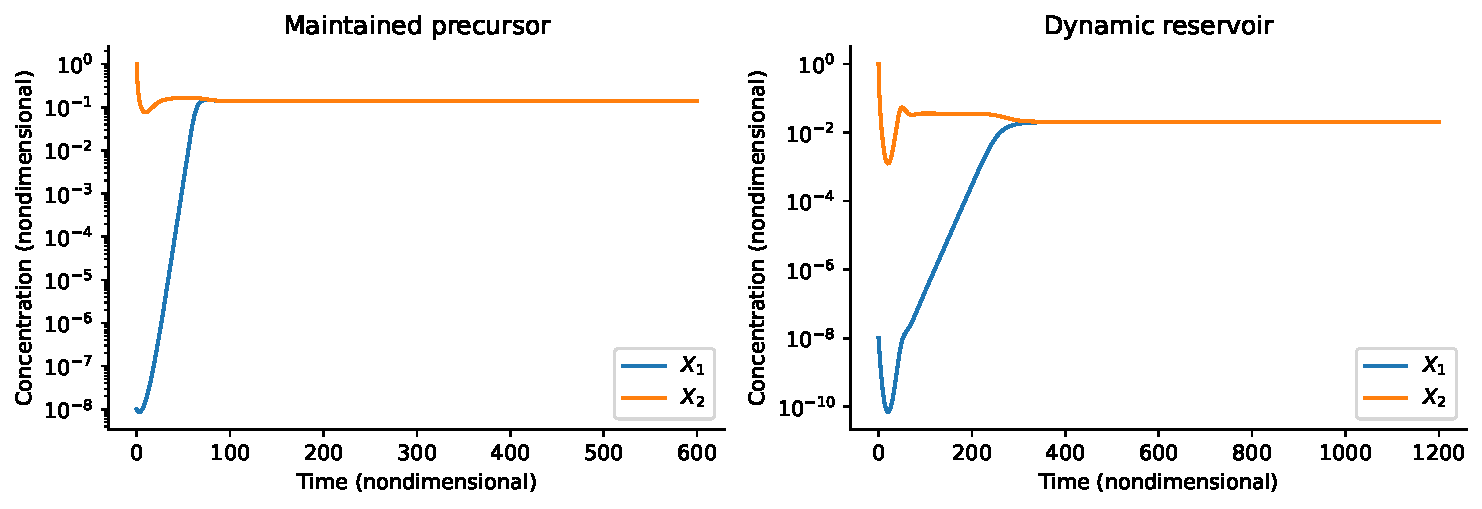
\includegraphics[width=\linewidth]{rare_recovery.pdf}
\caption{Numerical recovery of an initially rare consumer in the two reference systems ($n=2$). These trajectories illustrate Theorem~\ref{thm:roots}; they do not estimate its uniform floor or prove equilibrium convergence.}
\label{fig:rare}
\end{figure}
\begin{figure}[htbp]\centering
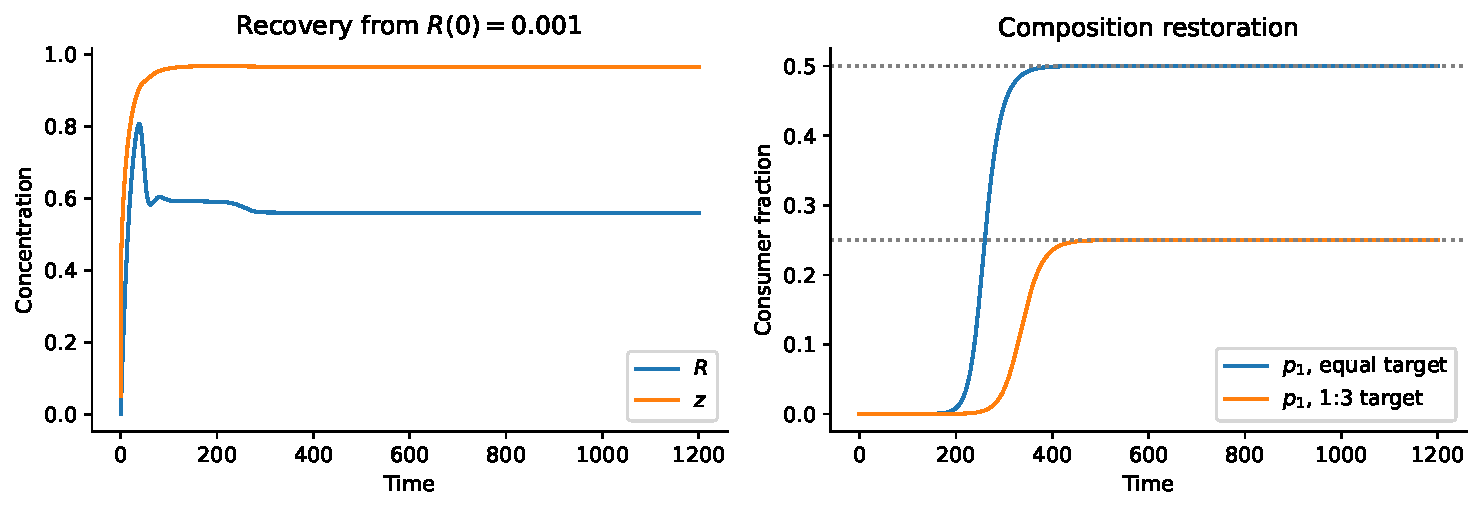
\includegraphics[width=\linewidth]{depleted_composition.pdf}
\caption{Left: reservoir $R$ and resource $z$ during recovery from $R(0)=0.001$ in system B. Right: consumer fraction $p_1$ for the equal target ($\rho=(2,2)$) and the prescribed $1{:}3$ target ($\rho=(4,4/3)$) of Theorem~\ref{thm:unequal}; both have $\kappa=1$ and the same total.}
\label{fig:depleted}
\end{figure}

The computed operating state of system B is
\[
\begin{aligned}
(A,B,z,H)&\approx(12.76381063,\,20.23476257,\,0.96519417,\,8.65272051),\\
(R,S)&\approx(0.56017133,\,0.04067410),
\end{aligned}
\]
with copying uptake $J=d(1-R)\approx0.02199143$. Thus about $43.98\%$ of the reservoir inflow enters copying and $56.02\%$ leaves as washout of unused $R$; these fractions refer only to the reservoir balance. With the $1{:}3$ target the computed consumers are approximately $(0.01016853,0.03050558)$ at the same total operating state.

\begin{figure}[htbp]\centering
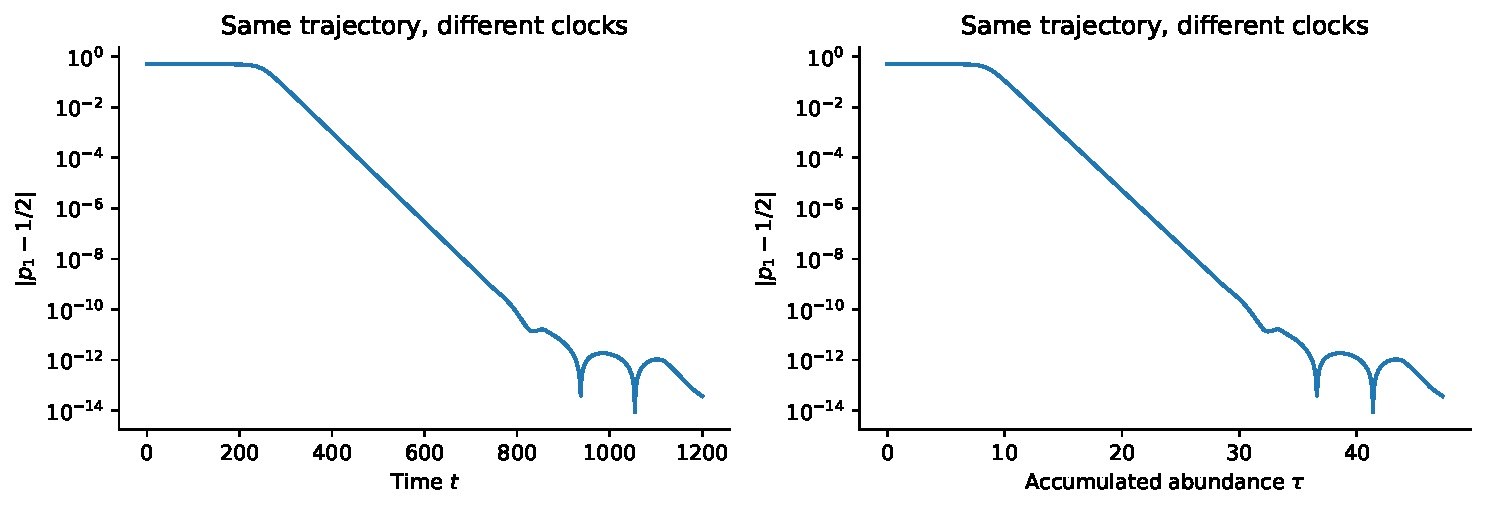
\includegraphics[width=\linewidth]{composition_clock.pdf}
\caption{Composition error $|p_1-\tfrac12|$ for the reference system B trajectory in physical time (left) and in accumulated abundance $\tau=\int S$ (right), the clock of \eqref{eq:p}. The final near-roundoff portion is numerical.}
\label{fig:clock}
\end{figure}
\begin{figure}[htbp]\centering
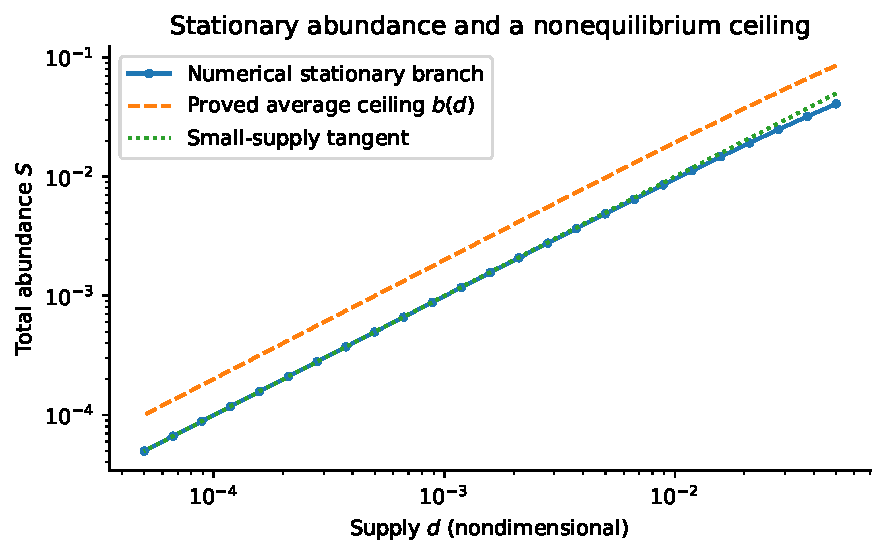
\includegraphics[width=.78\linewidth]{supply_scaling.pdf}
\caption{A numerical continuation of positive stationary states of system B, the proved ceiling $b(d)$ on the time-averaged total abundance from Theorem~\ref{thm:supply}, and the small-supply tangent $S_*'(0)d$ of Proposition~\ref{prop:branch}. Only a neighborhood of $d=0$ is covered by that proposition; the plotted continuation is not certified as a global branch.}
\label{fig:supply}
\end{figure}

Figure~\ref{fig:clock} shows the linear-in-$\tau$ decay predicted by \eqref{eq:rquant}: in accumulated abundance the composition error is a straight line on a logarithmic scale, whereas in physical time it is delayed while $S$ is still small. Figure~\ref{fig:supply} compares the stationary branch with the nonequilibrium ceiling; the stationary total lies below $b(d)$ throughout the computed range, as it must, since a constant solution has $\avg S=S_*$.

\begin{proof}[Proof of Proposition~\ref{prop:local}]
See Appendix~\ref{app:local}, where the ellipsoid, the rational matrix and the certified inequalities are listed and the argument (a quadratic Lyapunov function with interval bounds on the Jacobian, and a Newton--Kantorovich contraction for the equilibrium) is given.
\end{proof}
Proposition~\ref{prop:local} is an exact rational certificate with a conventional analytic proof, not a formally verified theorem. It supplies a concrete tolerance and initial-condition set with a floor of practical magnitude, in contrast to the global constants of Theorem~\ref{thm:roots}. It does not certify that either plotted trajectory enters $\cE$ at a particular time, and it does not replace the global proof.

\section{Discussion}\label{sec:discussion}

\paragraph{What the theorems say about coexistence.}
The mechanism is the classical one, intraspecific regulation stronger than interspecific regulation \cite{Chesson2000,LobryHarmand2006}, but the resource environment is not. The resource $z$ is produced by an interacting network under load, with no equilibrium response and no monotone dependence on the load assumed; in system B it must additionally be paired with a precursor that the consumers themselves deplete. The proof shows that the two familiar ingredients, resource-mediated competition and per-species density dependence, suffice for permanence even in this environment, provided the resource network satisfies a dissipation-versus-favorability inequality of the type \eqref{eq:donor}. Proposition~\ref{prop:negative} confirms that without density dependence the same environment gives competitive exclusion.

\paragraph{Structure of the argument.}
Three features of the proof may be useful elsewhere. (i) The resident network is analysed under a scalar load with no information about the load's dynamics, so the same resident lemma serves every consumer model whose coupling is through $-zL$. (ii) The bounded correction Lemma~\ref{lem:corrector} needs a potential that is bounded and whose derivative pays for unfavorable growth, not a Lyapunov function that decreases. (iii) The quotient comparison of Lemma~\ref{lem:recovery} converts a total floor into individual floors without classifying boundary dynamics, at the price of a floor that is linear in the total floor and inversely proportional to the number of consumers; Theorem~\ref{thm:composition} shows that this $1/n$ order is correct for the normalized family.

\paragraph{Physical interpretation and non-claims.}
The network is externally supplied through the maintained feeds of $A$ and $B$ and the effective channels $z\rightleftarrows H$ and $2z\rightleftarrows H$, which cannot both conserve positive resident molecular masses without omitted species. System B makes one copying precursor dynamic; it does not complete an atom-balanced or autonomous apparatus. The copying channel in system B is an effective trimolecular mass-action step; an elementary implementation would require explicit intermediates and a justified reduction. Positive deterministic concentrations do not establish survival at finite molecule or cell counts. The positive loss flux $\mu_iX_i+\rho_iX_i^2$ is not harvested product unless a collection channel is specified.

For dimensionalization choose a concentration scale $C_*>0$ and a time scale $t_*>0$; the conversion is consistent across the source (Table~\ref{tab:units}). For illustration only, $C_*=1\,\mu$M and $t_*=1\,$h convert $d=0.05$ to an exchange rate of $0.05\,\mathrm h^{-1}$ and an inflow of $0.05\,\mu\mathrm M\,\mathrm h^{-1}$, and the computed copying flux to $0.02199\,\mu\mathrm M\,\mathrm h^{-1}$. These are chosen units, not measured parameters.

\begin{center}
\captionof{table}{Dimensionalization with a common concentration scale $C_*$ and time scale $t_*$.}
\label{tab:units}
\begin{tabular}{lll}\toprule
Quantity&Dimensional value&Units\\\midrule
Concentration $x$&$C_*x$&concentration\\
Time $t$&$t_*t$&time\\
Feed $a,b,f$&$C_*(a,b,f)/t_*$&concentration/time\\
Unimolecular rate $k$&$k/t_*$&time$^{-1}$\\
Bimolecular rate $k$&$k/(C_*t_*)$&concentration$^{-1}$time$^{-1}$\\
Trimolecular rate $k$&$k/(C_*^2t_*)$&concentration$^{-2}$time$^{-1}$\\
Flux $J$&$C_*J/t_*$&concentration/time\\\bottomrule
\end{tabular}
\end{center}

\paragraph{Open problems.}
Three questions are left open. First, a global all-trajectory floor proportional to the supply $d$ as $d\to0$: the stationary branch has this scale, but transferring it to all trajectories would need a dynamical estimate that the present correction, whose constant $b_0=288/d_-$ grows as $d_-\to0$, does not give. Second, global convergence of the reactor, or a classification of the reduced block $J_{\rm red}$, beyond the local certificate. Third, the extension from scalar self-limited consumers to vector-valued consumer modules, and ultimately to structurally identified autocatalytic subnetworks, where the quotient comparison of Section~\ref{sec:sharp} is no longer available in closed form.

\paragraph{Formal verification.}
The formal development uses Lean~4.30.0 with a frozen mathlib manifest. Its five source endpoints include the equality between the encoded mass-action reaction list and the polynomial field, actual positive global solutions, and the eventual floors. Verification rejects warnings and admits no \texttt{sorry}; the reported axioms are only \texttt{Classical.choice}, \texttt{Quot.sound} and \texttt{propext}. The endpoint audit matches $82$ distinct source hashes. The sharpened recovery, the composition consequences and the negative control are separately compiled against the same source interfaces. Appendix~\ref{app:evidence} distinguishes these kernel-checked claims from the conventional proofs and the rational certificates. Neither an audit hash nor a numerical run is offered as a substitute for a proof.

\appendix
\section{Construction and verification of the resident estimate}\label{app:donor}
This appendix proves Lemma~\ref{lem:donor}. No convergence theorem for the resident network is an input. Work on $0\le A\le34$, $2\le B\le34$, $0\le z\le12$, $0\le H\le1536/7$ (which contains the region \eqref{eq:residentbox}). Define
\[
a_e(B)=\frac{2(33-B+eB)}{1+\sqrt{1+4e(33-B+eB)}},\quad
T_e(B)=B+a_e(B),\quad c=T_e'(B)=\frac{e(1+2a_e(B))}{1+2ea_e(B)} .
\]
The discriminant is positive and $ea_e^2+a_e=33-B+eB$, so $T_e(B)$ is the value of $A+B$ at which $A'+B'$ vanishes. Direct bounds give $-1\le a_e\le33$, $|c|\le1/500$, and, for $a_0=1+e(A+a_e)$, $99/100\le a_0\le101/100$. Put
\begin{align*}
r&=A+B-T_e(B),& F&=60-(2+z)B,\\
Z&=T_e(B)-(1+z)B-16z-4z^2+3H,& K&=16z+2z^2-hH .
\end{align*}
Writing $\ell(z)=\log(z+1)-\log(z+2)$, let $\phi(H)$ be the nonnegative root of $16\phi+2\phi^2=hH$, explicitly
\[
\phi(H)=\frac{2hH}{16+\sqrt{256+8hH}},\qquad0\le\phi(H)\le12 .
\]
Choose primitives with derivatives
\[
U'(z)=\frac{16z+4z^2}{(z+1)(z+2)},\qquad
P_e'(B)=-\log(60/B)+T_e'(B)\,\ell(60/B-2),\qquad
G'(H)=3\ell(\phi(H)) ;
\]
all integrands are continuous on the relevant intervals, and additive constants are immaterial. Set
\begin{equation}\label{eq:potential}
\widetilde V=B\log(z+2)-T_e(B)\ell(z)+U(z)-3H\ell(z)+P_e(B)+G(H)+\tfrac12r^2 ,
\end{equation}
and center it at $(A,B,z,H)=(0,2,0,0)$ to obtain $V_e$.

\subsection{Dissipation by divided differences}
In the unloaded network, exact substitution gives
\[
B'=F+a_0r,\qquad z'=Z+r,\qquad H'=K,\qquad r'=-a_0(1+c)r-cF .
\]
The gradient of \eqref{eq:potential} in the coordinates $(B,z,H,r)$ is
\[
\Bigl(\log(z+2)-c\,\ell(z)+P_e'(B),\ -\frac Z\omega,\ 3[\ell(\phi(H))-\ell(z)],\ r\Bigr),\qquad\omega=(z+1)(z+2).
\]
The mean value theorem supplies $m,\nu$ with the first component equal to $-mF$ and the third equal to $-\nu K$, where
\[
\tfrac1{500}\le m\le\tfrac{13}{50},\qquad\nu\ge\tfrac1{4000},\qquad2\le\omega\le182 .
\]
For the first, apply the mean value theorem to $(\log(t+2)-c\,\ell(t))/B$ between $t=z$ and $t=60/B-2$; along that segment $t+1\ge13/17$ and $4\le B(t+2)\le476$, while the derivative is $(1-c/(t+1))/[B(t+2)]$. For the third, $1/182\le\ell'\le1/2$ on $[0,12]$ and $K=(z-\phi)[16+2(z+\phi)]$.

Thus the unloaded derivative of $\widetilde V$ is
\[
-mF^2-\frac{Z^2}\omega-\nu K^2-a_0(1+c)r^2-(a_0m+c)rF-\frac{rZ}\omega ,
\]
which the exact square decomposition
\begin{align*}
&-\frac m2F^2-\frac{Z^2}{2\omega}-\nu K^2
-\Bigl(a_0(1+c)-a_0^2m-\frac{c^2}m-\frac1{2\omega}\Bigr)r^2\\
&\qquad-m\Bigl(\frac F2+a_0r\Bigr)^2-\frac{(mF/2+cr)^2}m-\frac{(Z+r)^2}{2\omega}
\end{align*}
bounds from above. The coefficient of $r^2$ is at least $\tfrac14$, by
\[
a_0(1+c)\ge\tfrac{99}{100}\cdot\tfrac{499}{500},\qquad
a_0^2m\le\bigl(\tfrac{101}{100}\bigr)^2\tfrac{13}{50},\qquad
\frac{c^2}m\le\tfrac1{500},\qquad\frac1{2\omega}\le\tfrac14 .
\]
We obtain $V_e'\le-\D_e$ with
\begin{equation}\label{eq:D}
\D_e=\tfrac14r^2+\tfrac1{1000}F^2+\tfrac1{364}Z^2+\tfrac1{4000}K^2 .
\end{equation}
A load $-zL$ in the resource equation changes the derivative by $(Zz/\omega)L$. On the box $Z\le2000$ and $0\le z/\omega\le1/5$, so this is at most $400L$.

\subsection{A low-resource residual gap}
For $0\le z\le3/4$ the response identity gives $T_e\ge33-1089/50000$. The polynomial
\begin{align*}
P_0(z)={}&(33-1089/50000-23/100)(z+2)\cdot20001-60(1+z)\cdot20001\\
&-(16z+4z^2)(z+2)\cdot20001+30000(16z+2z^2)(z+2)
\end{align*}
has, with $t=3/4-z\ge0$, the expansion
\[
P_0(z)=\tfrac{32094021}{200000}+\tfrac{3944380089}{50000}t+74967t^2+20004t^3\ge0 .
\]
Substituting $F,Z,K$ into the exact identity
\begin{align*}
&(z+2)\cdot20001\Bigl(Z+|F|+\tfrac32|K|-\tfrac{23}{100}\Bigr)\\
&\qquad=P_0(z)+(z+2)\cdot20001\,(T_e-33+1089/50000)\\
&\qquad\quad+20001\bigl[(1+z)F+(z+2)|F|\bigr]+(z+2)\bigl[\tfrac{60003}2|K|-30000K\bigr],
\end{align*}
every term on the right is nonnegative, so $|Z|+|F|+\tfrac32|K|\ge\tfrac{23}{100}$. Weighted Cauchy--Schwarz gives
\[
\bigl(|Z|+|F|+\tfrac32|K|\bigr)^2\le10364\bigl(\tfrac1{364}Z^2+\tfrac1{1000}F^2+\tfrac1{4000}K^2\bigr),
\]
hence $\D_e\ge529/103640000$. If $z\le3/4$, this bound together with $z\ge0$ gives $z-\tfrac12+C\D_e\ge\tfrac14$ with $C=150000$; if $z\ge3/4$, nonnegativity of $\D_e$ suffices. This proves the third inequality in \eqref{eq:donor}.

\subsection{Uniform potential and perturbation bounds}
The four gradient components in the coordinates $(B,z,H,r)$ have absolute bounds $140$, $1000$, $18$ and $67$ respectively, and $|c|\le1/500$; these follow from the divided differences above, $|F|\le536$, $|Z|\le2000$ and $|r|\le67$. Along the line segment from the centering point to the physical state, the first four physical coordinate speeds have absolute value at most $384$ and the speed of $r$ is at most $1200$. The potential variation is therefore bounded by
\[
140\cdot384+1000\cdot384+18\cdot384+67\cdot1200<10^6=K_0 ,
\]
which proves the centered bound $|V_e|\le K_0$.

At fixed actual load, every resident-rate error is a sum of at most ten signed rate errors times monomials bounded by $2000$ on the box, stoichiometric coefficients included. At radius $10^{-18}$ each physical derivative error is at most $10^{-13}$. Substituting into the gradient expression gives a potential derivative error at most $10^{-7}$ (the elementary estimate is in fact much smaller). This proves the perturbation clause and completes Lemma~\ref{lem:donor}.

\section{Exact local operating certificate}\label{app:local}
Use the full state $x=(A,B,z,H,R,X_1,X_2)\in\R^7$. All $21$ rates are independent, ordered as in \eqref{eq:rates} with $(k_1,\mu_1,\rho_1,k_2,\mu_2,\rho_2,f,w)$ appended to the thirteen resident rates. Let $r_0$ be the reference rates at $e=10^{-5}$, $d=1/20$, and let $F_r$ be the polynomial field at rates $r$. The exact rational center is
\[
\begin{gathered}
c=10^{-13}(127638106330396,\,202347625659673,\,9651941703983,\\
86527205137315,\,5601713297463,\,203370509477,\,203370509477).
\end{gathered}
\]
Define the symmetric rational matrix $P=10^{-9}M$, where
\begin{center}\scriptsize
\setlength{\tabcolsep}{3pt}
\begin{tabular}{rrrrrrr}
1026298486&-507128910&2060379318&3015248881&-1528107325&-2902025242&-2902025242\\
-507128910&988545587&-2001858258&-2924197933&1476664351&2808922060&2808922060\\
2060379318&-2001858258&5855388798&8806642948&-4475616469&-8445422819&-8445422819\\
3015248881&-2924197933&8806642948&13459291457&-6834866969&-12937422442&-12937422442\\
-1528107325&1476664351&-4475616469&-6834866969&9205238173&3717403038&3717403038\\
-2902025242&2808922060&-8445422819&-12937422442&3717403038&75141618542&62848784117\\
-2902025242&2808922060&-8445422819&-12937422442&3717403038&62848784117&75141618542
\end{tabular}
\end{center}
Put $p_-=1/\norm{P^{-1}}_\infty$, $p_+=\norm P_\infty$ and $r_b=10^{-5}$. The initial-condition set of Proposition~\ref{prop:local} is exactly
\begin{equation}\label{eq:ellipsoid}
\cE=\{x:(x-c)^TP(x-c)\le p_-r_b^2\},
\end{equation}
so its specification does not rely on rounded spectral values.

The rational verification interface is as follows. Let $J_0=DF_{r_0}(c)$ and $Q_0=-(PJ_0+J_0^TP)$. Exact Sylvester minors prove $P>0$. Let $q_-$ be the minimum over rows of the diagonal entry of $Q_0$ minus the sum of the absolute off-diagonal entries in that row. Exact interval evaluation over $\norm{x-c}_\infty\le r_b$ and $\norm{r-r_0}_\infty\le10^{-14}$ gives the conservative bounds of Table~\ref{tab:certificate}; all decimal endpoints there are rational bounds, and the accompanying certificate file contains the unreduced exact values.

\begin{table}[htbp]
\centering
\caption{Certified rational bounds for the local operating certificate.}
\label{tab:certificate}
\begin{tabular}{ll}\toprule
Quantity&Certified bound\\\midrule
$p_-$&$>0.007375$\\
$p_+$&$<168.802$\\
$q_-$&$>0.9999998$\\
$D_J=\sup\norm{DF_r(x)-J_0}_\infty$&$<0.000161829$\\
$F_c=\sup\norm{F_r(c)}_\infty$&$<4.142\cdot10^{-12}$\\
$q_--6p_+D_J$&$>0.83609$\\
$\norm{J_0^{-1}}_\infty D_J$&$<0.012897$\\
$\ell=0.006610005\le\sqrt{p_-/p_+}$&exact squared check\\
$(q_--6p_+D_J)\,\ell r_b-6p_+F_c$&$>5.10\cdot10^{-8}$\\\bottomrule
\end{tabular}
\end{table}

\begin{proof}[Proof of Proposition~\ref{prop:local}]
For symmetric positive $P$, $p_-I\le P\le p_+I$, so $\cE$ lies inside the box $\norm{x-c}_\infty\le r_b$, and on its boundary $\norm{x-c}_2\ge\ell r_b$. For $h=x-c$, Taylor's integral formula and $\norm A_2\le\sqrt7\norm A_\infty<3\norm A_\infty$ give
\[
\frac{\dd}{\dd t}(h^TPh)\le-(q_--6p_+D_J)\norm h_2^2+6p_+F_c\norm h_2 .
\]
The last inequality of Table~\ref{tab:certificate} makes this strictly negative on the boundary of $\cE$, so $\cE$ is forward invariant for every admissible rate vector. Its consumer floor is $c_6-r_b=c_7-r_b=0.0203270509477$.

For existence and uniqueness of the equilibrium, the map $N_r(x)=x-J_0^{-1}F_r(x)$ is a contraction on the box with Lipschitz constant $k=\norm{J_0^{-1}}_\infty D_J<1$, and exact arithmetic verifies $\norm{J_0^{-1}}_\infty F_c+kr_b<r_b$, so $N_r$ maps the box into itself. Banach's theorem gives a unique equilibrium in the box, at infinity-norm distance at most $\norm{J_0^{-1}}_\infty F_c/(1-k)$ from $c$; the certificate verifies that three times this bound is less than $\ell r_b$, placing the equilibrium strictly inside $\cE$. Finally the same Jacobian inequality, applied to the difference from this equilibrium along a segment in the convex box, gives strict quadratic decay in the $P$-norm, so every solution starting in $\cE$ converges to it.
\end{proof}

The certificate was found by floating-point computation (a Lyapunov equation for $P$, a Newton solve for $c$) and then checked in exact rational arithmetic; radii $10^{-3}$ and $10^{-4}$ fail the derivative bound and rate tolerances above $10^{-14}$ fail the boundary margin at radius $10^{-5}$. These failures locate the limits of this particular certificate, not an instability.

\section{Theorem-to-evidence map and reproducibility}\label{app:evidence}
All Lean declarations below are in the namespace \lean{MultiConsumerPermanence}; sources are under \lean{proofs/MultiConsumerPermanence/} and strict receipts are in the campaign workspace named at the end of this appendix. Compilation uses the repository verification bridge with warnings treated as errors.

\begin{center}\small
\begin{tabular}{>{\raggedright\arraybackslash}p{.17\linewidth}>{\raggedright\arraybackslash}p{.45\linewidth}>{\raggedright\arraybackslash}p{.29\linewidth}}\toprule
Statement&Lean declaration&Receipt\\\midrule
Thm~\ref{thm:roots} A1&\lean{reference_multi_species_permanence}&\lean{Main.verify.json}\\
Thm~\ref{thm:roots} A2&\lean{robust_multi_species_permanence}&\lean{RateMain.verify.json}\\
Thm~\ref{thm:roots} B1&\lean{reservoir_multi_species_permanence}&\lean{ReservoirMain.verify.json}\\
Thm~\ref{thm:roots} B2&\lean{robust_reservoir_multi_species_permanence}&\lean{ReservoirRateMain.verify.json}\\
Thm~\ref{thm:roots} B3&\lean{reservoir_supply_operating_limits}&\lean{SupplyMain.verify.json}\\
Lemma~\ref{lem:recovery}&\lean{variable_speed_eventual_bound}\newline\lean{sharp_species_floor}&\lean{SharpRecovery.verify.json}\\
Thm~\ref{thm:sharp}&\lean{sharp_reference_source_floor}\newline\lean{sharp_reservoir_source_floor}\newline\lean{sharp_robust_source_floor}\newline\lean{sharp_robust_reservoir_source_floor}&\lean{SharpSourceRecovery.verify.json}\\
Thm~\ref{thm:composition}, ratio limit (system A)&\lean{reference_pairwise_ratio_limit}&\lean{CompositionConsequences.verify.json}\\
Zero-face invariance; diagonal lift&\lean{reference_consumer_zero_face}\newline\lean{equal_composition_lift}&\lean{CompositionConsequences.verify.json}\\
Prop.~\ref{prop:negative}&\lean{no_individual_limitation_extinction_control}\newline\lean{unregulated_total_upper}&\lean{NegativeControl.verify.json}\\\bottomrule
\end{tabular}
\end{center}

The five endpoint declarations each assert the literal mass-action equality of the encoded reaction list with the polynomial field, the existence of a global positive solution from every positive initial state, and the eventual floor. The sharp recovery declarations reuse the established aggregate bounds and source derivative predicates; positive global existence remains supplied by the original roots. The negative control is connected to the literal perturbed field at its own rate vector.

Conventional proofs in this paper, not formalized: the quantitative integral estimate \eqref{eq:rquant}, the $n$-independent floor \eqref{eq:nscale}, the spectral factorization \eqref{eq:spectrum}, Theorem~\ref{thm:unequal}, the averaged bounds \eqref{eq:avgbalance}--\eqref{eq:budgets} (the pointwise extinction and the necessary bound \eqref{eq:necessary} are in B3), Proposition~\ref{prop:branch}, Proposition~\ref{prop:local}, and the construction of Appendix~\ref{app:donor} (whose inequalities are those used by the formal resident modules inherited from the single-consumer donor proof). The two rational certificates (donor enclosure, local ellipsoid) are reproducible arithmetic evidence for the stated conventional interfaces and have not been imported as kernel certificates.

Reproduction. The campaign workspace \lean{problem_workspaces/RAF_permanence_with_multiple_extinctions_dynamic_limiting_reservoirs/} contains the strict receipts, the endpoint audit (\lean{FINAL_ENDPOINT_AUDIT.json}, $82$ source hashes, toolchain \lean{leanprover/lean4:v4.30.0}), the script \lean{publication_experiments.py} that produces the four figures, the CSV trajectories, the stationary continuation and the two exact JSON certificates in about three seconds on one BLAS thread, and the historical ledger. The paper folder contains \lean{check_paper.py}, which replays in exact arithmetic every identity and constant printed here, checks the certificate values of Appendix~\ref{app:local} and Section~\ref{sec:branch} against the JSON files, and re-hashes the Lean sources against their receipts.

\bibliographystyle{plainnat}
\bibliography{refs}
\end{document}
